\section{Background}
\label{ch:background}

This chapter serves to explain the foundations of natural language processing (NLP), especially the subpart of
language modeling, needed to understand the problem and methodology used in this thesis. The two main building blocks
of this thesis are the examination of a state-of-the-art language model (LM) and its ability to generate high quality,
human-like text on the one hand and methods to distinguish such generations from human written text on the other hand.
In order to understand the problem and methodology used in this thesis, this chapter explains the foundations
of NLP (ch.~\ref{sec:history_of_language_modeling}), especially the subpart of language
modeling, and the foundations of deep learning (ch.~\ref{sec:deep_learning}) especially under the aspect of sequence
classification.

\subsection{History of language modeling}
\label{sec:history_of_language_modeling}

Natural language processing (NLP) is “an area of research and application that explores how computers can be used to
understand and manipulate natural language text or speech to do useful things”~\footcite{doi:10.1002/aris.1440370103}.
The applications of NLP such as speech recognition, sentiment analysis,
question answering and others are numerous~\footcite{DBLP:journals/corr/GattK17}.
Moreover, these applications are already being heavily used by industry and
consumers alike e.g. in the forms of digital voice assistants, sentiment analysis for recommender systems
and browser search bars~\footcite{8012330,10.1145/3064663.3064672,GoogleSearch}. The subcomponent of NLP
needed when it comes to tasks like machine translation, predictive typing or summarization that involve either
generating text or estimating the probability of text is called language modeling. The following notation mostly
follows the one from the CS224 Stanford Natural Language Processing with Deep Learning lecutre by Chris Manning~\footnote{\url{https://web.stanford.edu/class/cs224n/index.html}}.

Language modeling is the task of predicting “what word comes next“. More formally, this means:
Given a sequence of words $ x^{(1)}, x^{(2)}, \dots, x^{(t)} $, compute the probability of the next word $ x^{(t+1)} $:
\begin{equation}
    P(x^{(t+1)} | x^{(t)}, \dots, x^{(1)})
\end{equation}
where $ x^{(t+1)} $ can be any word in the vocabulary $ V = \{w_1, \dots, w_{|V|}\} $  \\
Having a system that does allows us to assign a probability to a snippet of text of length $ T $:
\begin{align}
    \begin{split}
    P(x^{(1)}, \dots, x^{(T)}) &= P(x^{(1)}) \times P(x^{(2)} | x^{(1)}) \times \cdots \times P(x^{(T)} | x^{(T-1)}, \dots, x^{(1)}) \\
    &= \prod_{t=1}^{T} P(x^{(t)} | x^{(t-1)}, \dots, x^{(1)})
    \end{split}
\end{align}
Developing and improving language models is a task central to language understanding by which we can measure how well machine learning systems actually comprehend natural language. This is demonstrated by the fact that “often (although not always), training better language models improves the underlying metrics of the downstream task (such as word error rate for speech recognition, or BLEU score for translation), which makes the task of training better LMs valuable by itself”~\footcite{DBLP:journals/corr/JozefowiczVSSW16}. \\
Since the first significant language model was proposed back in 1980~\footcite{880083}, language models and their architectures have gone through many changes. Especially the rise of Deep Learning and new network models such as RNNs or Transformers have fueled language modeling research in the past few years. The following chapters will cover word representation as the foundation for language models (ch.~\ref{sub:word_representation}) followed by the most common and most used language model types and architectures (ch.~\ref{sub:n_gram_models} - ch.~\ref{sub:neural_language_models}).

\subsubsection{Word representation}
\label{sub:word_representation}

The starting point for most NLP related tasks lies within the preprocessing of the textual input data. These must first be converted into a semantically meaningful numerical representation to allow for effective computation. The simplest way to represent a word numerically is by treating words as \textit{one-hot} vectors. Using this format, one word is encoded into an $ n $-dimensional vector of numbers where $ n $ is the vocabulary size and each entry takes on the value $ 0 $ except for the one that corresponds to the indexed word which takes on the value $ 1 $. This process generates very sparse feature vectors for each input word, which is no problem for simple classification tasks, but is unsuitable for larger problems as the dimension size increases for each word added to the vocabulary. Another issue of one-hot vectors is the fact that these representations hold no notion of similarity: If we take a look at the representations for the words “plane“ and “airplane“ we would get two vectors that are orthogonal, just as any two vectors in the whole vocabulary. This poses a problem as every word's similarity to other words is the same and we can not encapsulate the meaning of the word. Yoav Goldberg writes in his primer on neural networks for language processing that one-hot vectors should only be considered for problems where the model has only a small amount of input features, the inputs do not have to share model parameters and where there is a lot of data to learn from~\footcite{DBLP:journals/corr/Goldberg15c}.

Otherwise, the currently dominant approach in the field is to use word embeddings as feature vectors. Word embeddings follow the so called “distributional semantics“, which state that a word's meaning is given by the words that tend to occur in a similar context. This idea of context-dependent nature of meaning was first introduced by english linguist J.R. Firth~\footnote{\url{https://web.stanford.edu/class/linguist236/materials/ling236-handout-05-09-vsm.pdf}} with the famous quote:

\begin{quote}
  You shall know a word by the company it keeps.
\end{quote}

Following this idea we represent each word by a distribution of weights across many dimensions. Now, instead of having a one-to-one mapping between an element in the vector and a word, the representation of a word is spread across all of the entries in the vector, and each element in the vector contributes to the definition of many words. Having this new form of word vectors allows us to capture meaningful semantic and syntactic regularities between words in an expressive way. A simple way to illustrate this is depicted in figure~\ref{fig:word2vec_king_queen_composition}. \\
Here, our word vectors contain the knowledge that the difference between a “king“ and a “queen“ primarily lies within the gender of a person. Thus, if we subtract the word vector of “man“ from “king“ and we add the word vector of “woman“ we get a word vector that is very similar to the one of “queen“.

\begin{figure}[h]
  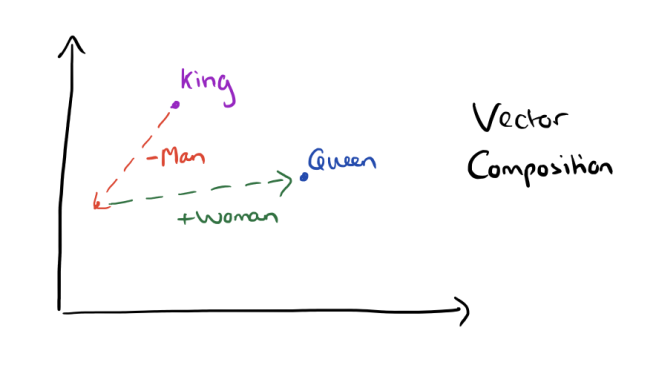
\includegraphics[height=5cm]{img/word2vec-king-queen-composition}
  \caption{Word2vec king queen composition}
\label{fig:word2vec_king_queen_composition}
\end{figure}

The most famous realization of these embeddings was introduced by the researchers of Google around Tomas Mikolov in their paper “Distributed Representations of Words and Phrases and their Compositionality“~\footcite{DBLP:journals/corr/MikolovSCCD13}. Hereafter, their proposed approach, Word2Vec, along with their used notation will briefly be presented, as its core ideas are found throughout other popular word embedding frameworks as well. \\
Given a sequence of training words $ w_1, w_2, \dots, w_T $, the objective (paragraph~\ref{par:cost_function}) is to minimize the average negative log likelihood
\begin{equation}
	\label{eqn:skip_gram_objective_function}
	J(\theta) = - \frac{1}{T} \sum_{t=1}^{T} \sum_{\substack{-m \leq j \leq m \\ j \neq 0}} \text{log} \ P(w_{t+j} | w_t; \theta)
\end{equation}
where $ m $ is the fixed window size containing the context words around the center word $ w_j $. Enlarging this window size results in more training examples and can lead to a higher accuracy, at the expense of training time. In order to compute the term $ P(w_{t+j} | w_t; \theta) $ a regular softmax function (ch 3.3.3 [HARDCODED, ref to softmax function]) can be applied
\begin{equation}
	\label{eqn:skip_gram_conditional_probability}
	P(o | c) = \frac{\text{exp} \ (u_{o}^{T} v_{c})}{\sum_{w \in V} \text{exp} \ (u_{w}^{T} v_c)}
\end{equation}
where we use two vectors per word $ w $: $ v_w $ when $ w $ is a center word and $ u_w $ when $ w $ is a context word. Optimizing the objective function results in high-quality distributed vector representations. It should be noted that for computational efficiency modified versions of these functions such as negative sampling or hierarchical softmax are used, as the presented ones do not scale well.

Even though word2vec embeddings are a powerful representation they do face certain limitations, which is why \textit{Stanford University}~\footnote{\url{https://www.stanford.edu}} took it upon itself to create an improved variant called GloVe~\footcite{pennington-etal-2014-glove}. While word2vec ignores that some context words appear more ofthen than others, GloVe stresses the importance of frequencies of co-occurrences and that these should not be “wasted“ as additional training examples. Therefore, GloVe builds word embeddings in a way that a combination of word vectors relates directly to the probability of these words' co-occurrence in the corpus. \\
Another alternative to word2vec is \textit{fasttext} by Facebook, which generates word vectors that generalize better, need less training data and can be trained “on more than one billion words in less than ten minutes using a standard multicore CPU, and classify half a million sentences among 312K classes in less than a minute“ according to the authors~\footcite{DBLP:journals/corr/JoulinGBM16}. FastText also takes word parts into account, i.e. FastText not only stays on a word level of depth but also goes into the character level.


\subsubsection{N-Gram models}
\label{sub:n_gram_models}

One solution in dealing with the problem of predicting a word after a sequence of $ (n - 1) $
words in the form of a Markov model, i.e. the probability of each event depends only on the state
attained through the previous event, is called an n-gram model. An “n-gram” hereby denotes a chunk 
of n consecutive words. The core idea is that the probability of a word $ w_i $ occurring in the 
$ i^{th} $ instance after a sequence of $ (i - 1) $ preceding words can be approximated by observing 
only the preceding context of $ (n - 1) $ words.

Following this insight we can compute the probability of all n-grams in a corpus of text by simply counting their occurrences.
Doing so allows us to calculate the conditional probabilities like so:
\begin{align}
    \begin{split}
        P(x^{(t+1)} | x^{(t)}, \dots, x^{(1)}) &= P(x^{(t+1)} | x^{(t)}, \dots, x^{(t - 2 + 2)}) \\ \\
        &= \frac{P(x^{(t+1)}, x^{(t)}, \dots, x^{(t - 2 + 2)})}{P(x^{(t)}, \dots, x^{(t - 2 + 2)})} \\ \\
        &\approx \frac{\text{count}(x^{(t+1)}, x^{(t)}, \dots, x^{(t - n + 2)})}{\text{count}(x^{(t)}, \dots, x^{(t - n + 2)})}
    \end{split}
\end{align}
N-gram models where $ n = 1 $, $ n = 2 $ and $ n = 3 $ are called unigram, bigram and trigram, respectively. The parameter $ n $ typically does not get bigger than $ 5 $. Having the conditional probabilites new text can be generated by conditioning on the provided input. After getting a probability distribution over the vocabulary a sampling strategy (ch. 3.3.3 [HARDCODED]) that returns a word has to be applied.

Even though n-gram models have been widely used especially due to their simplicity and scalability they do face certain limitations that have led to a decrease in their popularity. One problem that can occur is the one of unexpected n-grams: if the $ n $-gram encountered in the test setting did not appear in the corpus that the model was trained on, then the probability for the $ n^{th} $ word conditioned on the $ (n-1) $ words is $ 0 $. If an $ (n-1) $-gram is encountered in the test setting but not in the training data, then the model can not calculate the probability of any word that comes after. These two sparsity limitations can, however, partly be encountered by using smoothing and backoff techniques. The storage problem is evident, as increasing $ n $ or simply enlarging the training corpus increases the model size, which poses a significant problem for larger NLP applications. The implications of this restriction can be withdrawn from the following illustrative generated text snippet:

\begin{quote}
“today the price of gold per ton , while production of shoe lasts and shoe industry , the bank intervened just after it considered and rejected an imf demand to rebuild depleted european stocks , sept 30 end primary 76 cts a share”
\end{quote}

Because of the inability to expand the context window effectively, we remain tied to a LM that can generate grammatical but also incoherent model that can not relate predictions to history reaching further into the past. N-gram language models are still widely used in speech recognition due to their high efficiency in inference~\footcite{wang2019improving} but their limitations caused by poor generalization to unobserved n-grams and inability to capture long range dependencies led to the rise of neural language models.





\subsubsection{Neural language models}
\label{sub:neural_language_models}

\paragraph{Neural network}
This is some text.

\paragraph{Recurrent neural networks}
This is some text.

\paragraph{Convolutional neural networks}
This is some text.

\paragraph{Attention and transformers}
This is some text.

\subsection{Deep Learning}
\label{sec:deep_learning}

This is deep learning.
